\chapter{State of the Art}
Aktuell gibt es in der Bewegungsforschung von Robotern mit mehreren Beinen drei vorherrschende Ansätze \cite{simmering2023walknet}:
\begin{itemize}
    \item \textbf{Central Pattern Generators} (sind Oszilatorsysteme oder neurale Netze, die eine rhythmische Ausgabe erzeugen, ohne eine bestimmte Eingabe vorauszusetzen.)
    \item \textbf{lernende Ansätze} (darunter fällt auch der in dieser Arbeit thematisierte Reinforcement Learning Ansatz)
    \item \textbf{sensorbasierte Ansätze} (sind besser erklärbar im Vergleich zu lernenden Ansätzen. Normalerweise sind sie relativ anpassbar an sich verändernde Umgebungen.)
\end{itemize}
Simmering et al. \cite{simmering2023walknet} erforschen fortgeschrittene Laufmethoden der sensorbasierten Walknet-Architektur und sehen vor allem ein Potenzial in der Verbindung mehrerer dieser Ansätze.

Während Machine Learning in den letzten Jahren erfolgreich auf viele Aufgaben angewandt wurde, treffen lernende Ansätze in der Anwendung bei realen, mehrbeinigen Robotern -- welche kontinuierlichen Kontroll-Aufgaben darstellen -- noch auf einige Probleme \cite{schilling2020decentralized}.
Einerseits werden Roboter aus Praktikabilitäts- und Sicherheitsgründen meist in Simulationen trainiert.
(Häufig werden auch zunächst in der Simulation Grundsteine gelegt und dann die daraus gewonnenen Modelle manuell für eine bestimmte Aufgabe feingeschliffen \cite{schilling2020decentralized}.)
In der Folge kann allerdings der Transfer auf reale Probleme erschwert werden, da etwa in der realen Anwendung deutlich mehr (Signal-)Rauschen von Eingabesensoren auftritt, was zur Hinterfragung führt, ob tatsächlich ein fester \ac{mdp} vorliegt \cite{schilling2020decentralized}.
Andererseits ist es ein fundamentales Problem, dass beim (Deep) Reinforcement Learning gelernt wird, den Reward möglichst gut auszunutzen, weshalb diese Art von Lernproblemen zu Overfitting neigt.
Das bedeutet, dass Deep Reinforcement Learning dazu tendiert, Nischenlösungen zu finden, die meist nicht dazu in der Lage sind, adaptiv auf neue, vor allem unvorhergesehene Situationen zu reagieren \cite{schilling2020decentralized}.

Schilling et al. \cite{schilling2020decentralized} schlagen deshalb einen dezentralisierten Ansatz vor, der dem Nervensystem von Insekten ähnelt (\autoref{fig:insect}).
Im Gegensatz zu \cite{waidner.2020} wird dabei nicht ein zentraler Controller verwendet, der alle Beine steuert und sämtliche Zustandsinformationen erhält, sondern jedes Bein wird durch einen eigenen Controller mit reduzierten Zustandsinformationen gesteuert.
Vorteilhaft ist hieran vor allem, dass die Komplexität/Dimensionalität des Problems deutlich verringert wird verglichen mit Ansätzen, die einen zentralen Controller verwenden.
Versuche resultierten in der Erkenntnis, dass die erzielten Resultate mit beiden Algorithmen ähnlich gut ausfielen.
Jedoch hatte der dezentrale Ansatz eine rapide, fast halbierte Trainingszeit, um dieses Ergebnis zu erreichen \cite{schilling2020decentralized}.
Verwendet wurde in beiden Fällen der \ac{ppo}-Algorithmus, welcher in der aktuellen Forschung allgemein gute Ergebnisse bei kontinuierlichen Problemen liefert, ohne dabei extensive Anpassungen der Hyperparameter zu erfordern \cite{schilling2020decentralized}.
Im Kontext dieser Arbeit ist festzustellen, dass der im Experiment verwendete Roboter über deutlich mehr und detailliertere Eingangsdaten verfügte, die unter anderem über Sensoren gesammelt wurden (z.B. auch Sensoren für Bodenkontakt der Beine und Körperneigung).
Aufgrund der sehr eingeschränkten Informationen, die dem Roboter in dieser Arbeit zur Verfügung stehen, scheint die Verfolgung eines dezentralen Ansatzes leider nicht erfolgversprechend.

\begin{figure}
    \centering
    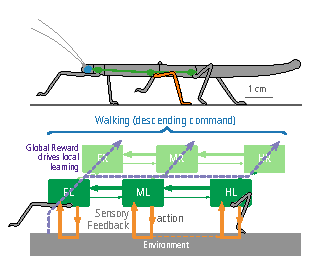
\includegraphics[width = 0.35\textwidth]{Bilder/decentralized-insect.pdf}
    \caption{Dezentrale Architektur in Anlehnung an Stabinsekten \cite{schilling2020decentralized}}
    \label{fig:insect}
\end{figure}

% \hrule
% \begin{itemize}
%     \item \enquote{Decentralized Deep Reinforcement Learning for a Distributed and Adaptive Locomotion Controller of a Hexapod Robot}
%     \item Machine Learning in letzten Jahren erfolgreich auf viele Aufgaben angewandt
%     \item DRL scheint noch Probleme zu haben bei der Anwendung für reale Roboter in \enquote{continuous control tasks}
%     \item vor allem im Umgang mit unvorhergesehenen Situationen gibt es Probleme
    
%     \item ursprünglich aus Bereich Computerspiele, deshalb viel in simulierten Umgebungen
%     \item Transfer auf reale Probleme kann schwierig sein (\enquote{nature of such problems is fundamentally different from those in playing computer games})
%     \item häufig wird zunächst die Simulation genutzt, um Grundsteine zu legen, die dann manuell feingeschliffen werden für eine bestimmte Aufgabe
%     \item zwei fundamentale Probleme: soll den Reward ausnutzen, neigt deshalb zu Overfitting; reale Anwendungen deutlich mehr (Signal-)Rauschen, führt zu Hinterfragen von festem Markov Decision Process
%     \item DRL tendiert dazu, Nischenlösungen zu finden, die meist nicht dazu in der Lage sind, adaptiv auf neue Situationen zu reagieren
    
%     \item Tendenz geht dahin, hierarchische oder dezentralisierte Ansätze zu verfolgen
%     \item hierarchisch erlaubt flexibles wechseln zwischen verschiedenen Unteraufgaben und Verhaltensweisen und somit auch Agieren in verschiedenen Kontexten möglich, bislang allerdings nur mit geringen Freiheitsgraden umgesetzt
%     \item Fokus diesen Papers eher auf Störungen und Varietät in einem spezifischen Kontext mit einem spezifischen Verhalten
    
%     \item PPO funktioniert allgemein gut mit kontinuierlichen Problemen ohne viel Hyperparameter-Tuning
%     \item Median-Geschwindigkeit einer Episode ist der Reward
%     \item \cite{schilling2020decentralized}
% \end{itemize}




% \hrule
% \begin{itemize}
%     \item \enquote{Adaptation of a Decentralized Controller to Curve Walking in a Hexapod Robot}
%     \item bei Robotern mit mehreren Beinen aktuell drei vorherrschende Ansätze
%     - Central Pattern Generators (CPGs)
%         - Oszilatorsysteme oder neurale Netze, die rhythmische Ausgabe erzeugen, ohne bestimmte Eingabe vorauszusetzen\\
%     - lernende Ansätze\\
%     - Sensorenbasierte Ansätze
%         - sind besser erklärbar verglichen mit lernenden Ansätzen
%         - normalerweise relativ anpassbar an sich verändernde Umgebungen
    
%     \item sehen Potenzial in Verbindung mehrerer Ansätze
%     \item \cite{simmering2023walknet}
% \end{itemize}


Tsounis et al. \cite{tsounis2020deepgait} verfolgen einen bislang komplett neuen Ansatz, der vor allem für die Fortbewegung in unwegsamen Gelände erfolgversprechend scheint.
Dabei ist die Idee, die Schrittplanung als Aufgabe von der eigentlichen Durchführung der Schritte abzukoppeln.
Dadurch können zwei unabhängige Modelle trainiert und verwendet werden, die jeweils eine deutlich geringere Dimension haben, als es bei einem gemeinsamen Überproblem der Fall wäre.
Außerdem bieten solche Ansätze die Möglichkeit, einzelne Komponenten unabhängig voneinander zu optimieren und auszutauschen.
Weiterhin evaluieren Tsounis et al. für das Training der Schrittplanung nur die physikalische Machbarkeit der Schritte, anstatt die Umgebung vollständig zu simulieren.
Dabei ist eine deutlich höhere Genauigkeit bei weniger Rechenaufwand möglich, als wenn die Simulation eines Schritts Frame für Frame geladen und evaluiert würde.
Die erzielten Resultate sind weit besser als die von vergleichbaren Ansätzen -- insbesondere für das Überwinden von Klüften.
Allerdings ist dazu auch anzumerken, dass die Modelle auf dem Terrain trainiert wurden, auf das sie später angewandt wurden.
Dennoch konnte eine gute Verallgemeinerung festgestellt werden.
Ein wichtiges Fazit der Arbeit war, dass eine ausreichend hohe Entropie während des Trainings maßgeblich für den Gesamterfolg verantwortlich ist.

% \hrule
% \begin{itemize}
%     \item \enquote{DeepGait: Planning and Control of Quadrupedal Gaits using Deep Reinforcement Learning}
%     \item Kombination von state-of-the-art modellbasierten Methoden der Bewegungsplanung und Reinforcement Learning
%     \item Evaluieren die physikalische Machbarkeit anstatt physisch zu simulieren
%     \item trennen Schrittplanung und Ausführung
%     \item es können ganze Schritte evaluiert werden und nicht nur einzelne Frames einer Simulation
%     \item Hauptproblem in Schrittplanung ist Kombinatorik, wegen der vielen möglichen Kombinationsmöglichkeiten für Kontaktpunkte mit dem Untergrund
%     \item aber: Training auf späterem Terrain, allerdings relativ gute Verallgemeinerung
%     \item Entropie ist extrem wichtig
%     \item Weit bessere Resultate als andere Ansätze, gerade was das Überbrücken von Klüften angeht
%     \item \cite{tsounis2020deepgait}
% \end{itemize}

Abschließend soll hier noch der Ansatz von Smith et al. \cite{smith2023learning} erwähnt werden.
Die Idee hier ist, agile und komplexe Bewegungsfähigkeiten durch Übertragung von Lernerfahrungen zu erlernen und anzupassen.
Der Hintergrundgedanke beruht darauf, dass selbst einfache Aufgaben schon sehr komplex modulierte Reward-Funktionen benötigen können, um eine gezielte Bewegung zu erhalten.
Wenn nun eine noch deutlich komplexere Bewegungsform von Null trainiert wird, kann dies teilweise fast unmöglich zu bewältigen sein, da nur ein sehr bestimmtes Verhalten Reward nach sich ziehen kann.
Für ein spezifisches Zielproblem zu trainieren mag zwar scher sein, doch häufig ist es zumindest möglich, mit einfacheren Trainingsumgebungen und Problemen zumindest relevante Daten zu erhalten, welche für einen Lernprozess von Interesse sind.
So sollen Daten von beliebigen Trainingsprozessen transformiert und transferiert werden können, um neue Fähigkeiten einfacher und in einem Bruchteil der Zeit erlernen zu können (\autoref{fig:transfer}).
Zum Beispiel können Daten von einem Roboter, der gelernt hat, auf zwei Beinen zu stehen, dabei helfen, ihm das Laufen auf diesen zwei Beinen beizubringen.
Auch mit diesem Ansatz wurden bereits vielversprechende Ergebnisse erzielt.
Sollten sich die Versuche dieser Arbeit schwierig gestalten, so könnte es zukünftig interessant sein, einen solchen Ansatz zu erforschen, um die Bewältigung der komplexeren Aufgabenstellung im Vergleich zu \cite{waidner.2020} zu ermöglichen.

% \hrule
% \begin{itemize}
%     \item \enquote{Learning and Adapting Agile Locomotion Skills by Transferring Experience}
%     \item selbst einfache Aufgaben können sehr komplexe modulierte Reward-Funktionen benötigen, um die gezielten Bewegungen zu erhalten
%     \item Wenn eine Bewegungsform sehr gut koordinierte Bewegungen voraussetzt, kann sehr schwer sein, wenn man von Null beginnt (-> nur sehr konkretes Verhalten kann Reward nach sich ziehen)
%     \item Für ein spezifisches Zielproblem zu trainieren mag schwer sein, doch häufig ist es möglich, mit einfacheren Trainingsumgebungen zumindest relevante Daten zu erhalten, welche für einen Lernprozess von Interesse sind
%     \item (Aus auf Hinterbeinen stehen wird Laufen)
%     \item Häufig ist es schwierig, das in agileres Verhalten zu erweitern; insbesondere mit stark angepassten Reward-Funktionen, um das Verhalten überhaupt erst zu erzeugen
%     \item => Training Agiler Roboter Fähigkeiten erleichtern durch Transfer mit existierenden suboptimalen Fähigkeiten
%     \item \cite{smith2023learning}
% \end{itemize}

\begin{figure}
    \centering
    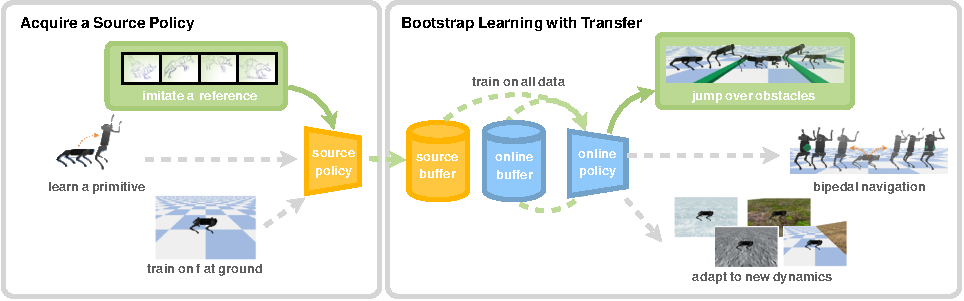
\includegraphics[width = 0.8\textwidth]{Bilder/transfer-learning.pdf}
    \caption{Transfer von Trainingsdaten zur Bewältigung komplexer Probleme \cite{smith2023learning}}
    \label{fig:transfer}
\end{figure}